\documentclass[10pt,journal,compsoc]{IEEEtran}

\usepackage{grffile}
\usepackage[dvips]{graphicx}

\usepackage[cmex10]{amsmath}

\hyphenation{}

\begin{document}

\title{Eficiencia del sistema de propulsi\'on WARP de la nave espacial USS Enterprise}


\author{Lucila Stancato,~\IEEEmembership{I.T.B.A,}
		Dami\'an Modernell,~\IEEEmembership{I.T.B.A,}
		Juan Brasca,~\IEEEmembership{I.T.B.A,}
		Conrado Negro,~\IEEEmembership{I.T.B.A}%

}

\IEEEcompsoctitleabstractindextext{%
\begin{abstract}
%\boldmath
Analizamos la eficacia en la generaci\'on de n\'umeros pseudo-aleatorios del generador de L'Ecuyer aplicando los tests $\chi^2$ y $KS$
, en los que determinamos la conveniencia de usar dicho generador. Tambi\'en realizamos la estimaci\'on del tiempo
de vuelo de la nave espacial USS Enterprise mediante la simulaci\'on de Montecarlo.
\end{abstract}

\begin{IEEEkeywords}
Generador de L'Ecuyer, n\'umeros pseudoaleatorios, simulaci\'on de Montecarlo, propulsor WARP
\end{IEEEkeywords}
}%\IEEEcompsoctitleabstractindextext

\maketitle

\IEEEdisplaynotcompsoctitleabstractindextext

\IEEEpeerreviewmaketitle

\section{Introducci\'on}

\IEEEPARstart{L}{}os dispositivos de c\'omputo no pueden generar n\'umeros aleatorios dado que 
son dispositivos deterministas. La \'unica manera de obtenerlos ser\'ia a trav\'es de un dispositivo
que detecte procesos naturales como por ejemplo el intervalo de tiempo entre dos part\'iculas $\alpha$
en una muestra radiactiva.\\
En la secci\'on 2 utilizamos y sometemos a prueba el generador propuesto por L'Ecuyer para la
generaci\'on de n\'umeros pseudoaleatorios que a diferencia de los n\'umeros aleatorios, pueden 
ser generados por una computadora. En las distintas pruebas determinamos la bondad de ajuste del
generador. En la secci\'on 3 utilizamos el modelo de simulaci\'on de Montecarlo de sistemas
distribuidos para determinar el tiempo medio de vuelo y varianza del USS Enterprise.\\
Comprobamos la efectividad del generador de L'Ecuyer ya que genera n\'umeros que aparentan ser 
aleatorios.
sdafasdfasdfasdfasdfasdfasdfasdfasdfasdfasdfasdf

\section{Generador de L'Ecuyer}
El generador propuesto por L'Ecuyer en 1998 combina dos generadores lineales congruenciales (LCGs)
seg\'un los pasos del 1 al 5:
\begin{itemize}
 \item{PASO 1:} Seleccionar una semilla $X_{1,0}$ en el rango $[1,2147483562]$ para el primer LCG y otra $X_{2,0}$ en el rango $[1,2147483398]$ para el segundo LCG.\\
 \item{PASO 2:} Evaluar cada generador individual:
 \begin{align*}
  X_{1,n+1} &= 40014 X_{1,n} mod 2147483563\\
  X_{2,n+1} &= 40692 X_{2,n} mod 2147483399
 \end{align*}
 
 \item{PASO 3:} Computar:
 \begin{equation*}
  X_{n+1} = (X_{1,n+1} - X_{2,n+1}) mod 2147483562
 \end{equation*}
 
 \item{PASO 4:} Computar:
  \begin{equation*}
  \label{eq:f(t)}
  U_{n+1} = \left\{
  \begin{array}{rl}
	\frac{X_{n+1}}{2147483563} \hspace{0.5cm} X_{n+1} > 0\\\\
	\frac{2147483562}{2147483563} \hspace{0.5cm} X_{n+1} = 0\\
  \end{array} \right.
  \end{equation*}

 \item{PASO 5:} Hcer $n = n + 1$ y volver al $PASO 2$
\end{itemize}

Los n\'umeros obtenidos por medio de este generador tienen una distribuci\'on uniforme.
Generamos 10000 n\'umeros que presentamos en el histograma de la figura 1.

\begin{figure}[t]
\label{fig:histogramalecuyer}
\begin{center}
\centering
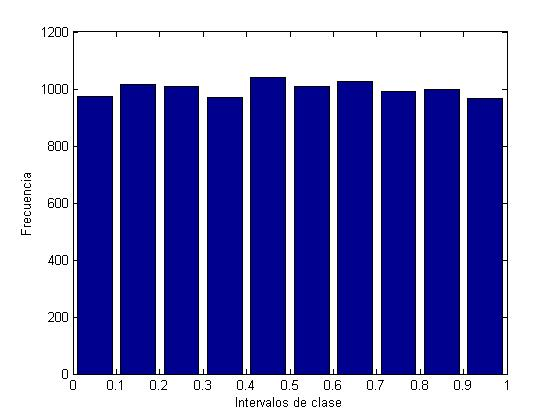
\includegraphics[width=3.2in]{clases.jpg}
\caption{10000 n\'umeros generados con el generador de L'Ecuyer divididos en 10 intervalos de clase que muestran una distribuci\'on uniforme}
\end{center}
\end{figure}

Analizamos gr\'aficamente en el plano las duplas $(U_i, U_{i+1})$ en la figura 2 y en el espacio las ternas $(U_i, U_{i+1}, U_{i+2})$ en la figura 3.

\begin{figure}[t]
\label{fig:2d}
\begin{center}
\centering
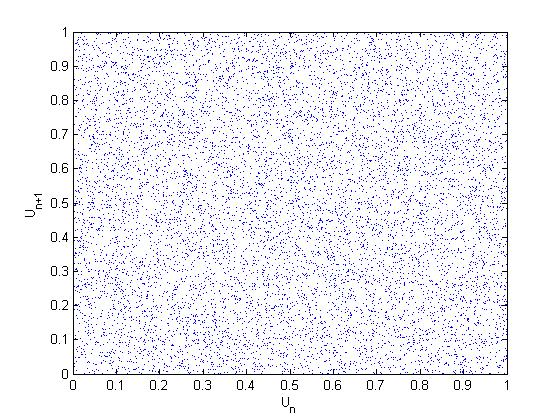
\includegraphics[width=3.2in]{2d_groso.jpg}
\caption{Observamos la distribuci\'on uniforme de los 10000 n\'umeros obtenidos con el generador de L'Ecuyer en el plano}
\end{center}
\end{figure}

\begin{figure}[t]
\label{fig:3d}
\begin{center}
\centering
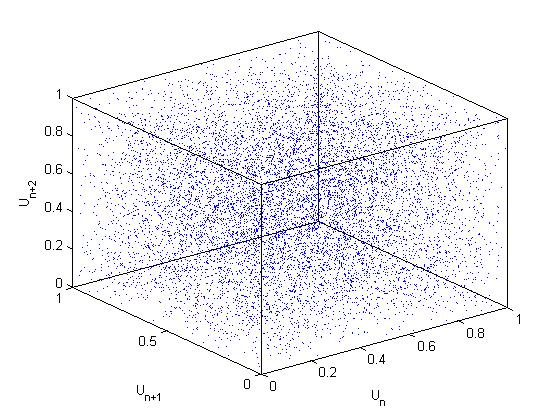
\includegraphics[width=3.2in]{3d.jpg}
\caption{Observamos la distribuci\'on uniforme de los 10000 n\'umeros obtenidos con el generador de L'Ecuyer en el espacio}
\end{center}
\end{figure}

\subsection{Prueba $\chi^2$}
En las figuras 2 y 3 observamos que la distribuci\'on parece ser uniforme, pero podemos usar
tests m\'as elaborados para corroborar esos resultados. El test $\chi^2$ determina, con un nivel
de significaci\'on $\alpha$ que determinamos en $5\%$ si es razonable suponer que la distribuci\'on 
observada de las 10000 muestras es consistente con que la variable tenga una distribuci\'on uniforme.
Las hip\'otesis del test son:
\begin{itemize}
 \item {$H_{0}$:} $\chi_{0}^2 < \chi_{n-1,\alpha}$ (Los n\'umeros obtenidos mediante el m\'etodo de L'Ecuyer est\'an uniformemente distribuidos)
 \item {$H_{1}$:} $\chi_{0}^2 \ge \chi_{n-1,\alpha}$ (Los n\'umeros obtenidos mediante el m\'etodo de L'Ecuyer no est\'an uniformemente distribuidos)
\end{itemize}
Para la prueba decidimos tomar 10 intervalos de clase, determinando as\'i 9 grados de libertad. Para estos
par\'ametros, el valor cr\'itico es $\chi_{n-1,\alpha}^{2} = 16.91898$. El estad\'istico $\chi_{0}^{2}$ se computa
mediante la f\'ormula de la ecuaci\'on 1

\begin{equation}
 \chi_{0}^{2} = \sum_{i=1}^{n} \frac{(O_i - E_i)^2}{E_i}
\end{equation}

y resulta $\chi_{0}^{2} = 5.592$ por lo que se acepta la hip\'otesis nula $H_0$.

\subsection{Prueba de Kolmogorov-Smirnov}
Las hip\'otesis utilizadas para esta prueba son:
\begin{itemize}
 \item {$H_{0}$:} $D < D_{\alpha}$ (Los n\'umeros obtenidos mediante el m\'etodo de L'Ecuyer est\'an uniformemente distribuidos)
 \item {$H_{1}$:} $D \ge D_{\alpha}$ (Los n\'umeros obtenidos mediante el m\'etodo de L'Ecuyer no est\'an uniformemente distribuidos)
\end{itemize}
Donde $D$ es el resultado de la prueba y $D_{\alpha}$ es el valor cr\'itico correspondiente a los par\'ametros de la prueba.
Computamos el valor $D$ con la f\'ormula de la ecuaci\'on 2.
\begin{equation}
 D = max(D^{+}, D^{-})
\end{equation}

siendo
\begin{align}
 D^{+} &= max(\frac{i}{n}-x_i)\\
 D^{-} &= max(x_i - \frac{i-1}{n})
\end{align}

donde $x_i$ es el i-\'esimo valor de los calculados por el m\'etodo de L'Ecuyer.
Realizando los c\'alculos, resulta $D = 0.0034$ y como $D_{\alpha} = 0.0136$,
tambi\'en se acepta la hip\'otesis nula.

\section{}

\section{algoritmo funcion triangular}

\section{Estimaci\'on del tiempo de vuelo medio del USS Enterprise}
La nave espacial USS Enterprise, famosa por las pel\'iculas de Star Treck, es impulsada por un sistema de propulsi\'on WARP, 
que se conforma por dos motores a los laterales, uno a babor y otro a estribor. Ambos propulsores son alimentados por un nucleo WARP
donde se llevan a cabo reacciones de aniquilaci\'on materia / antimateria, moderadas por cristales de dilitio. Dichos cristales 
son procesados en una c\'amara controlada, llamada Matriz de Dilitio.\\
El tiempo de operaci\'on de cada propulsor es una variable aleatoria de distribuci\'on exponencial con tiempo medio de 10 d\'ias. 
A su vez, el tiempo de operaci\'on entre fallos del n\'ucleo WARP es de 72 horas, pudiendo variar linealmente hasta en 12 horas. 
La nave puede propulsarce a velocidad WARP con un solo motor funcionando. Por \'ultimo, las c\'amaras de dilitio funcionan de forma tal que, la c\'amara principal tiene un tiempo de operaci\'on entre 
20 y 50 horas, de distribuci\'on uniforme. La c\'amara redundante tiene un tiempo entre fallos de 5 a 12 horas.\\
\indent Definimos dos variables aleatorias  $X_1$ y $X_2$, las cuales tienen una distribucui\'on de probabilidad uniforme y corresponden 
a la c\'amara principal, de tiempo de operaci\'on entre fallos de 20 a 50 horas, y a la c\'amara redundante de tiempo de 
operaci\'on entre fallos de 5 a 12 horas. Tambi\'en definimos una variable aleatoria $X_3$ de distribuci\'on 
triangular, que corresponde al n\'ucleo WARP, con par\'ametros $\alpha = 60$ horas, $\beta = 72$ horas y $\delta = 84$ horas. Adem\'as
definimos las variables aleatorias $X_4$ y $X_5$ de distribuci\'on exponencial, que corresponden a los propulsores WARP del Enterprise.
Ambas variables tienen un tiempo medio $T_1 = T_2 = $ 10 dias.\\

Observamos la representaci\'on del sistema de propulsi\'on de la nave Enterprise en la figura 4.


\begin{figure}[t]
\label{fig:3d}
\begin{center}
\centering
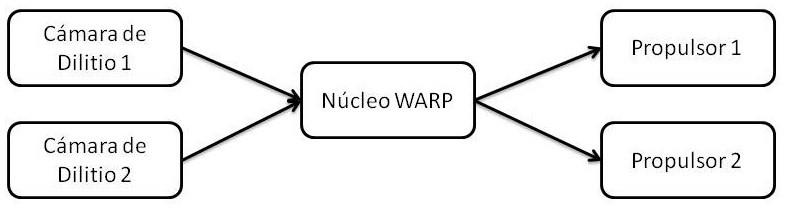
\includegraphics[width=3.2in]{propulsor.jpg}
\caption{Esquema de representaci\'on del sistema de propulsi\'on de la nave espacial USS Enterprise, donde el sistema falla, si falla el n\'ucleo WARP, o ambos propulsores, o ambas c\'amaras de dilitio ) }
\end{center}
\end{figure}

Para estimar el tiempo de vuelo del USS Enterprise, definimos una variable aleatoria $T$ que la definimos en (5).
\begin{equation}
T(i) = min( max(X_1, X_2), X_3, max(X_4, X_5) );
\end{equation}
%\begin{figure}[t]
%\label{fig:refuerzos2}
%\begin{center}
%\centering
%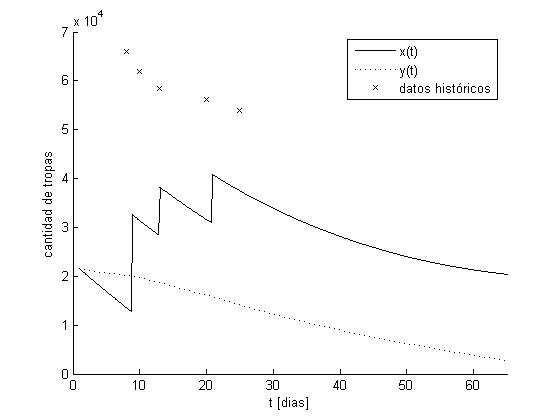
\includegraphics[width=3.2in]{grafico3_bis}
% where an .eps filename suffix will be assumed under latex, 
% and a .pdf suffix will be assumed for pdflatex; or what has been declared
% via \DeclareGraphicsExtensions.
%\caption{Segunda politica de refuerzos}
%\end{center}
%\end{figure}
%
%\begin{figure*}[!t]
%\centerline{\subfloat[Case I]\includegraphics[width=2.5in]{subfigcase1}%
%\label{fig_first_case}}
%\hfil
%\subfloat[Case II]{\includegraphics[width=2.5in]{subfigcase2}%
%\label{fig_second_case}}}
%\caption{Simulation results}
%\label{fig_sim}
%\end{figure*}

\section{Conclusi\'on}

\begin{thebibliography}{1}

\bibitem{IEEEhowto:kopka}
D\'iaz, A. R. \emph{El concepto de control}. Departamento de Ingenier\'ia Informatica. 
Instituto Tecnol\'ogico de Buenos Aires.
\end{thebibliography}

\end{document}


